%!TEX TS-program = pdflatex 
%!TEX encoding = UTF8
%!TEX spellcheck = en-US
%--------------------------
% to compile use "latexmk --pdf sup_MotionClouds.tex" 
%--------------------------
\documentclass[a4paper,11pt]{article}%draft
%-------definitions-----
\newcommand{\AuthorA}{Paula~Sanz Leon}%
\newcommand{\AuthorB}{Ivo~Vanzetta}%
\newcommand{\AuthorC}{Guillaume S.~Masson} %
\newcommand{\AuthorD}{Laurent U.~Perrinet}%
\newcommand{\AddressA}{INCM, CNRS / Aix-Marseille University, France}
\newcommand{\AddressB}{Institut de Neurosciences de la Timone, CNRS / Aix-Marseille University, Marseille, France}%
\newcommand{\Website}{https://laurentperrinet.github.io}%
\newcommand{\EmailA}{Paula.Sanz@univ-amu.fr}%
\newcommand{\EmailB}{Ivo.Vanzetta@univ-amu.fr}%
\newcommand{\EmailC}{Guillaume.Masson@univ-amu.fr}%
\newcommand{\EmailD}{Laurent.Perrinet@univ-amu.fr}%
\newcommand{\Title}{%
Supplementary Material to : \\ %
Motion Clouds: Model-based stimulus synthesis of natural-like random textures for the study of motion perception}%

%\newcommand{\Title}{%
%Supporting Information to : \\ %
%Motion Clouds: Model-based stimulus synthesis of natural-like random textures for the study of motion perception}%
%--------------------------

%% Packages
\usepackage[utf8x]{inputenc}
\usepackage[english]{babel}
\usepackage{natbib}
\usepackage[pdftex]{graphicx} 
\usepackage{graphics} 
\usepackage{amssymb,amsmath,bm,amsfonts}
\usepackage[usenames,dvipsnames]{color}
\usepackage{float}
\usepackage[pdftex,colorlinks=true,linkcolor=black]{hyperref}
\usepackage{multirow}
\usepackage{subfigure}
\usepackage{tabularx}
\usepackage{colortbl}
\usepackage{color}
\usepackage{booktabs}
\usepackage{fullpage}
\usepackage{times}
\usepackage{amsmath,bm}
\usepackage{tikz}
\usepackage{listings}
\usepackage{fancyvrb}
\usepackage{verbatim}
\usepackage{alltt}
\usepackage{watermark}
\usepackage{fullpage}
%\usepackage{fourier}
\usepackage{nicefrac} 
\usepackage{units}
\usepackage{authblk}
%\usepackage[notablist,notabhead]{endfloat}
\makeatletter
\renewcommand{\@makecaption}[2]{%
\vskip\abovecaptionskip
\hbox to \hsize{\hfil #1\hfil}%
\vskip\belowcaptionskip}
\makeatother
\usetikzlibrary{calc,3d}
\usetikzlibrary{shapes,arrows}
%\captionsetup{margin=10pt,labelfont=bf}
%\usepackage[on]{auto-pst-pdf}
%\usepackage{pstricks,multido,fp,pst-coil,pst-text}
%\usepackage{pst-3dplot}

%\usepackage{movie15}

%% Declarations and definitions

 %new float to avoid putting the tables at the end when using endfloat package
\floatstyle{plain}
\newfloat{mytable}{thp}{lop}
\floatname{mytable}{Table}


\definecolor{light-gray}{gray}{0.95}
\DeclareGraphicsExtensions{.jpg,.pdf,.png,.tiff}%.bmp,.mps,
\graphicspath{{results/}}
\hypersetup{
 unicode=false, % non-Latin characters in Acrobat�??s bookmarks
	pdftitle={Supplementary Material: Motion Clouds},%
	pdfauthor={\AuthorA < \EmailA > \AddressB - \AuthorB < \EmailB > - \AuthorC < \EmailC > - \AuthorD < \EmailD > },% \Website},% 
	%pdfkeywords={\Keywords},%
	%pdfsubject={\Acknowledgments}%
 pdfcreator={LaTeX}, 	% creator of the document
 pdfproducer={LUP,PSL}, 			% producer of the document
 colorlinks=true, % false: boxed links; true: colored links
 linkcolor = Black, 	% color of internal links
 citecolor = Black, 	% color of links to bibliography
 filecolor = Black, 			 % color of file links
 urlcolor = Black 		 % color of external links
}
\lstset{ %
language=Python, % the language of the code
basicstyle=\footnotesize, % the size of the fonts that are used for the code
numbers=left, % where to put the line-numbers
numberstyle=\footnotesize, % the size of the fonts that are used for the line-numbers
stepnumber=1, % the step between two line-numbers. If it's 1, each line 
 % will be numbered
numbersep=5pt, % how far the line-numbers are from the code
%backgroundcolor=\color{light-gray}, % choose the background color. You must add \usepackage{color}
%commentstyle=\color{gray}, % white comments
stringstyle=\ttfamily , % typewriter type for strings
showstringspaces=false, % no special string spaces
showspaces=false, % show spaces adding particular underscores
showstringspaces=false, % underline spaces within strings
showtabs=false, % show tabs within strings adding particular underscores
frame=single, % adds a frame around the code
tabsize=2, % sets default tabsize to 2 spaces
captionpos=b, % sets the caption-position to bottom
breaklines=true, % sets automatic line breaking
breakatwhitespace=false, % sets if automatic breaks should only happen at whitespace
title=\lstname, % show the filename of files included with \lstinputlisting;
 % also try caption instead of title
escapeinside={\%*}{*)}, % if you want to add a comment within your code
%morekeywords={*,...} % if you want to add more keywords to the set
}
\lstset{morecomment=[s][\color{blue}]{"""}{"""}}
\bibpunct{(}{)}{;}{a}{}{;}
\setlength{\parindent}{0in}
\setcounter{secnumdepth}{-1}  % this line turn off the section numbering

% Title Page
\title{\Title}%
\date{}%
\author[1,2]{\AuthorA \thanks{\EmailA}}
\author[1,2]{\AuthorB \thanks{\EmailB}}
\author[1,2]{\AuthorC \thanks{\EmailC}}
\author[1,2]{\AuthorD \thanks{Corresponding Author, \EmailD}}% , \Website}}
\affil[1]{\AddressA}
\affil[2]{\AddressB}

%\newcommand{\skipme}[1]{} % #1
%
%\newcommand{\hgid}{null}
%\def\baselinestretch{1.3}%
%\usepackage{lineno}
%\linenumbers
%\setpagewiselinenumbers
%\newcommand{\HRule}{\rule{\linewidth}{0.5mm}}

\begin{document}
\maketitle
\vspace{-1cm}

%%%%%%%%%%%%%%%%%%% Include files %%%%%%%%%%%%%%%%%%%%%%%%%%%%%%

%\input{MotionCloudsSupplementary}

%!TEX root = sup_MotionClouds.tex
%!TEX TS-program = pdflatex 
%!TEX encoding = UTF8
%!TEX spellcheck = en-US

\section{Computer implementation using Python}
In this part, we will briefly describe how Motion Clouds can be implemented while taking into account technical constraints such as discretization and videographic displays. We will also outline the algorithm used to generate our calibrated motion clouds using Python libraries. %

\subsection{Defining Fourier units, discrete units and physical units}\label{subsub:Normalised_Units}
In vision research, stimulus parameters depend on experimental conditions such as viewing distance and other properties of the display, such as the refreshing rate. Here, we will define the parameters of interest to implement when computing Motion Clouds based in the parameters showed in Table~\ref{table:units_experiment} where give a description of their physical values in one example experimental setup.

\begin{mytable}
\begin{center}
 \begin{tabular}{l l l l}
 \toprule
 Symbol  & Magnitude & Value & Unit \\
  \hline
 $D$    & Viewing distance distance & 570  & [mm]\\
 $X,Y$ & Stimulus size &  640 x 480 &[px] \\
$VA$\footnote   & Stimulus width in degrees of visual angle at viewing distance D & 38,1 &[deg] \\
$ f_{rate}$   & Frame rate  &  50 &[Hz] \\ 
$ T $   & Stimulus duration & 0.6 &[sec]\\
 \bottomrule
\end{tabular}
  \caption{Physical units in an optical imaging set-up.} 
  \label{table:units_experiment}
\end{center}
\end{mytable}

Both $N_X$ and $N_Y$ are determined by the frame (stimulus) size ($X$ and $Y$), while $N_{frame}$ is determined by the frame rate ($f_{rate}$) and the stimulus duration ($T$). These parameters define the stimulus' spatiotemporal periods. In this example we set $N_{frame}=30$. Additionally, velocities $V_x$ and $V_y$ have arbitrary units with the convention that if $V_x=1$, it means that average motion is equal to an average displacement of one spatial period over one temporal period and the same applies to $V_y$. (See Figure \ref{fig:movie_cube}).  
In line with this, we had introduced earlier the normalization factor $f_{t_0} =\frac{N_X}{N_{frame}}$. In the spatiotemporal domain implies that there is a translation of a distance $VA_X$ during a period $T$. We remind that degrees of visual angle are defined by $VA=2*\arctan\left(\unitfrac{S}{2D}\right)$, where $S$ is stimulus size on the screen ($X$ or $Y$) and $D$ is the viewing distance. 

\subsection{Defining stimulus and Fourier cubes}
Note first that the visual stimulus $\mathbf{I}$ is a real-valued function, therefore the inverse Fourier transform of our spectrum must be purely real, and its transform must be Hermitian. This means that the frequency component $(f_x,f_y,f_t)$ is the complex conjugate of the component at frequency $(-f_x,-f_y,-f_t)$. Therefore, there is no information in the negative frequency components that is not already available from the positive frequency components. 
To ensure that, the envelope will always be symmetric with respect to the origin in the Fourier domain, while the phase spectrum will be Hermitian by construction.  An alternative consists in taking the real part of the complex inverse Fourier transform of any envelope (symmetric or not). 
Note that by construction of the Fourier transform, stimuli are generated in the the 3D toroidal space and they are invariant up to displacement in multiples of the spatiotemporal period. As a consequence, there is no border or center and moreover any given Motion Cloud may be concatenated in space or time : For instance, playing a Motion Clouds movie in a loop is smooth and there is no abrupt transient. This property is useful to create large stimuli with limited resources by ''tiling'' a stimulus multiple times. Mathematically, a set of Motion Clouds is generated using normalized input arguments. First, we define the quantization of the Fourier space defined above in cubes of size $N_j, j \in {X,Y,frame}$, respectively for horizontal, vertical and time axis. 
In practice we will use the Fast Fourier Transform (FFT). As a consequence, the resulting stimulus cube will be of the same size as the frequency cube  and $N_j, j \in {X,Y,frame}$  should be preferentially defined as an integer power of two. Each frequency axis (in Cartesian coordinates ($f_{x}$, $f_{y}$ and $f_{t}$)) belongs always to the interval $[-0.5,0.5]$ although the number of points is different. The frequency resolution is given by $\left( \unitfrac{1}{N_X}, \unitfrac{1}{N_Y}, \unitfrac{1}{N_{frame}}\right)$ and $f_x,f_y,f_t=0.5$ (in \unitfrac{cyc}{px} ,\unitfrac{cyc}{px}, \unitfrac{cyc}{frame}) is the Nyquist frequency, i.e., the maximal frequency that can be represented without having undesirable aliasing effects. %~\citep{Scipy-ifftn}

\begin{figure}[h!]
%!TEX root = main_MotionClouds.tex
%!TEX TS-program = pdflatex 
%!TEX encoding = UTF8
%!TEX spellcheck = en-US
\tikzset{node distance=4cm, auto}
     
% fourier cube
\begin{center}
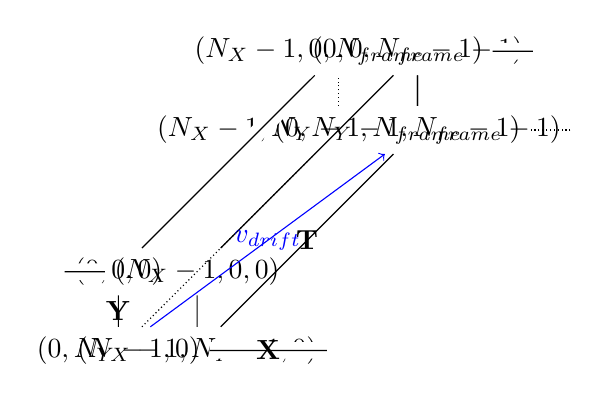
\begin{tikzpicture}[%
   back line/.style={densely dotted},
  cross line/.style={preaction={draw=white, -,line width=6pt}}]
  \node (A) {$(0,0,0)$};
  \node [right of=A] (B) {$(N_X-1,0,0)$};
  \node [below of=A] (C) {$(0,N_Y-1,0)$};
  \node [right of=C] (D) {$(N_X-1,N_Y-1,0)$};
 
  \node (A1) [right of=A, above of=A, node distance=2.8cm] {$(N_X-1,0,N_{frame}-1)$};
  \node [right of=A1] (B1) {$(0,0,N_{frame}-1)$};
  \node [below of=A1] (C1) {$(N_X-1,N_Y-1,N_{frame}-1)$};
  \node [right of=C1] (D1) {$(0,N_Y-1,N_{frame}-1)$};
 
  \draw[back line] (D1) -- (C1) -- (A1);
  \draw[back line] (C) -- (C1);
  \draw[cross line] (D1) -- (B1) -- (A1) -- (A)  -- (B) -- (D) to node [swap] {\textbf{X}} (C) to node [swap] {\textbf{Y}} (A);
  \draw (D)  to node [swap] {\textbf{T}} (D1) -- (B1) -- (B);
  \draw[->,color=blue] (C) to node [swap] {$v_{drift}$} (D1);  

  
\end{tikzpicture}
\end{center}
\caption{Motion Cloud cube: $V_x=1$ is defined as to produce an average displacement of $\dfrac{1}{N_X}$ per frame.}
\label{fig:movie_cube}
\end{figure}
In Figure \ref{fig:MC_flowchart} we show the flow chart of the sequential construction method. We begin by building a three dimensional matrix whose dimensions are given by the input arguments $N_{X}$, $N_{Y}$ and $N_{frame}$ so that $\mathcal{E}(f_x,f_y,f_t)\, \in \mathbb{R}^{N_X\times N_Y \times N_{frame}}$. The first two define the image size, width and height, respectively. The third dimension is the length of the image-series (number of frames). 

\begin{figure}%[h!]
\begin{center}
% Define the layers to draw the diagram
\pgfdeclarelayer{background}
\pgfdeclarelayer{foreground}
\pgfsetlayers{background,main,foreground}

% Define block styles
\tikzstyle{decision} = [diamond, draw, fill=white,
    text width=6em, text centered, node distance=2.5cm, inner sep=0pt]
\tikzstyle{block} = [rectangle, draw, fill=black!10,
    text width=12em, text centered, rounded corners, minimum height=4em]
\tikzstyle{line} = [draw, very thick, color=black!50, -latex']
\tikzstyle{cloud} = [draw, rectangle,fill=black!20, node distance=4.5cm,text width=8em, text centered, rounded corners, minimum height=4em]
\tikzstyle{decision answer}=[near start,color=black]
    
% todo@Paula : so it is not a sequence anymore... make the function independent?
\begin{tikzpicture}[node distance = 2.5cm, scale=0.5]
    % Place nodes
    \node [cloud] (init) {initialize \\Fourier grids};
    \node [cloud, left of=init, node distance=3.4cm] (expert) {experimental\\constraints}; % todo@Paula : table 1?
    \node [cloud, right of=init,node distance=3.4cm] (system) {stimulus input parameters\\ $N_X$,$N_Y$,$N_{frame}$};% todo@Paula : table 2?
    \node [block, below of=init, node distance=2.cm] (color) {build color envelope $\mathcal{C}_{\alpha}(f_{R})$};
    \node [block, below of=color,node distance=2.2cm] (sphere) {select a sphere $sf_0$ with a bandwidth $B_{sf}$\\ $\mathcal{G}(s_{f_0}, B_{sf})$};
    \node [block, below of=sphere] (speed) {select the speed plane with a thickness $B_V$ and speed $v_x$ or $v_y$\\$\mathcal{V}(V,B_V)$};
%    \node [decision, below of=speed,node distance=2.8cm] (orientation) {orientation tuning?};
%    \node [block, left of=orientation, node distance=4cm] (direction) {select envelope direction with peak orientation $\theta$\\$|F(\theta)|$};
    \node [block, below of=speed, node distance=2.8cm] (orientation) {select envelope direction with peak orientation $\theta$\\$\mathcal{O}(\theta,B_{\theta})$};
    \node [block, below of=orientation, node distance=2.5cm] (phase) {apply random phases \\ $e^{i\phi}$};
    \node [block, below of=phase, node distance=1.8cm] (ifft) {compute the IFFT};
    \node [block, below of=ifft, node distance=2.1cm] (rectify) {rectify the Motion Cloud (energy and contrast normalization)};
    \node [block, below of=rectify, node distance=2.1cm] (stop) {save stimulus \\(movie)};
    
    
    
    % Draw edges
    \path [line] (init) -- (color);
    \path [line] (color) -- (sphere);
    \path [line] (sphere) -- (speed);
    \path [line] (speed) -- (orientation);
%    \path[line] (orientation) -- node[decision answer] {yes} (direction);    
%    \path [line] (direction) |- (phase);
%    \path [line] (orientation) -- node {no}(phase);
    \path [line] (orientation) -- (phase);
    \path [line] (phase) -- (ifft);
    \path [line] (ifft) -- (rectify);
    \path [line] (rectify) -- (stop);
    \path [line,dashed] (expert) -- (init);
    \path [line,dashed] (system) -- (init);
    %\path [line,dashed] (system) |- (color);
    \path [line,dashed] (system) |- node {contrast} (rectify);
    
    % Draw background color layers
     \begin{pgfonlayer}{background}
     	% global box
        \path (expert.west |- system.north)+(-3,0.5) node (a) {};
        \path (system.east |- stop.south)+(+0.8,-0.3) node (c) {};    
        \path[fill=black!5,rounded corners, draw=black!50, dashed]    (a) rectangle (c); 
        
     	% sphere box
        \path (color.west |- color.north)+(-0.8,0.5) node (a) {};
        \path (orientation.east |- orientation.south)+(+0.8,-1.3) node (c) {};    
        \path[fill=blue!70!green!10,rounded corners, draw=black!50, dashed]   (a) rectangle (c); 
        
     	% speed box
        \path (speed.west |- speed.north)+(-0.5,0.3) node (a) {};
        \path (speed.east |- speed.south)+(+0.5,-0.3) node (c) {};          
        \path[fill=blue!10!green!10,rounded corners, draw=black!70, dashed]   (a) rectangle (c);  
            
     	% fft box
        \path (phase.west |- phase.north)+(-0.8,0.2) node (a) {};
        \path (ifft.east |- ifft.south)+(+0.9,-0.2) node (c) {};          
        \path[fill=red!20,rounded corners, draw=black!70, dashed]  (a) rectangle (c);                                                            
                                                                  
    \end{pgfonlayer}
    
\end{tikzpicture}
\caption{We show the Motion Clouds flow chart to summarize the main steps of the algorithm. The summary is in \ref{subsection:flowchart}}
\label{fig:MC_flowchart}
\end{center}
\end{figure}

\subsection{Summary: Flowchart}\label{subsection:flowchart}
 First, experimental parameters ( $N_{X}$, $N_{Y}$, $N_{frame}$) are initialized and physical units are normalized ($s_{f_0}$, $V_X$, $V_Y$).  Second, the color envelope is generated according to the parameter $\alpha$. Third, this color envelope ($\mathcal{C_{\alpha}}$) is multiplied by the global Fourier envelope constructed by the product of the speed ($\mathcal{V}$), spatial frequency ($\mathcal{G}$) and orientation envelopes ($\mathcal{O}$). The last step in the Fourier domain is to multiply the Fourier modulus by  a random phase ($e^{i\phi}$). Thus, after computing the 3-dimensional inverse Fourier transform we obtain a dynamic random phase texture, that is the Motion Cloud movie as a numpy array that can further be processed to be for example stored as a sequence of frames.


\subsection{Code example}
\label{subsection:implementation}

Motion Clouds are built using a collection of scripts that provides a simple way of generating complex stimuli suitable for neuroscience and psychophysics experiments. It is meant to be an open-source package  that can be combined with other packages such as PsychoPy or VisionEgg.%~\citep{Visionegg}\. \\~\citep{psychopy_a} 

All functions are implemented in one main script called \textit{MotionClouds.py} that handles the Fourier cube, the envelope functions as well as the random phase generation and all Fourier related processing. Additionally, all the auxiliary visualization tools to plot the spectra and the movies are included. Specific scripts such as \textit{test\_color.py}, \textit{test\_speed.py}, \textit{test\_radial.py} and \textit{test\_orientation.py} explore the role of different parameters for each individual envelope (respectively color, speed, radial frequency, orientation). Our aim is to keep the code as simple as possible in order to be comprehensible and flexible. To sum up, when we build a custom  Motion Cloud there are 3 simple steps to follow:

\begin{enumerate}
\item[1.] set the MC parameters and construct the Fourier envelope, then visualize it as iso-surfaces,
\end{enumerate}

\begin{lstlisting}
import MotionClouds as mc
import numpy as np
fx, fy, ft = mc.get_grids(mc.N_X, mc.N_Y, mc.N_frame) # define Fourier domain
envelope = mc.envelope_gabor(fx, fy, ft, V_X=1., V_Y=0., B_V=.1, sf_0=.15, B_sf=.1, theta=0., B_theta=np.pi/8, alpha=1.) # define an envelope
mc.visualize(fx, fy, ft, envelope)  # Visualize the Fourier Spectrum
\end{lstlisting}

\begin{enumerate}	
\item[2.] perform the IFFT and contrast normalization; visualize the stimulus as a 'cube' visualization of the image sequence,
\end{enumerate}

\begin{lstlisting}
movie = mc.random_cloud(envelope)
movie = mc.rectif(movie)
mc.cube(fx, fy, ft, movie, name=name + '_cube') # Visualize the Stimulus
\end{lstlisting} 

\begin{enumerate}
\item[3.] export the stimulus as a movie (.mpeg format available), as separate frames (.bmp and .png formats available) in a compressed zipped folder, or as a Matlab$^{\rm TM}$ matrix (.mat format). 
\end{enumerate}

\begin{lstlisting}
mc.anim_save(movie, name, display=False, vext='.mpeg')
\end{lstlisting}

If some parameters are not given, they are set to default values corresponding to a ''standard'' Motion Cloud. Moreover, the user can easily explore a range of different Motion Clouds simply by setting  an array of values for a determined parameter. Here, for example, we generate 8 MCs with increasing spatial frequency $s_{f_0}$ while keeping the other parameters fixed to default values:
%
\begin{lstlisting}
for sf_0 in [0.01, 0.05, 0.1, 0.2, 0.3, 0.4, 0.5, 0.6]:
	name_ = 'figures/' + name + '-sf_0-' + str(sf_0).replace('.', '_')
	mc.figures_MC(fx, fy, ft, name_, sf_0=sf_0) # function performing plots for a given set of parameters
\end{lstlisting}

Here, we show the source code of \textit{MotionClouds.py}. The test cases are available on request to the corresponding author. 

\begin{lstlisting}
#! /usr/bin/env python
# -*- coding: utf8 -*-
"""

Main script for generating Motion Clouds

(c) Laurent Perrinet - INT/CNRS

Motion Clouds (keyword) parameters:
size    -- power of two to define the frame size (N_X, N_Y)
size_T  -- power of two to define the number of frames (N_frame)
N_X     -- frame size horizontal dimension [px]
N_Y     -- frame size vertical dimension [px]
N_frame -- number of frames [frames] (a full period in time frames)
alpha   -- exponent for the color envelope.
sf_0    -- mean spatial frequency relative to the sampling frequency.
ft_0    -- spatiotemporal scaling factor. 
B_sf    -- spatial frequency bandwidth
V_X     -- horizontal speed component
V_Y     -- vertical speed component
B_V     -- speed bandwidth
theta   -- mean orientation of the Gabor kernel
B_theta -- orientation bandwidth
loggabor-- (boolean) if True it uses a log-Gabor kernel (instead of the traditional gabor) 

Display parameters:

vext       -- movie format. Stimulus can be saved as a 3D (x-y-t) multimedia file: .mpg movie, .mat array, .zip folder with a frame sequence.     
ext        -- frame image format.
T_movie -- movie duration [s].
fps      -- frame per seconds

"""

import os
DEBUG = False
if DEBUG:
    size = 5
    size_T = 5
    figsize = (400, 400)  # faster
else:
    size = 7
    size_T = 7
    figsize = (800, 800) # nice size, but requires more memory

import numpy as np
N_X = 2**size
N_Y = N_X
N_frame = 2**size_T
ft_0 = N_X/float(N_frame)
alpha = 1.0
sf_0 = 0.15
B_sf = 0.1
V_X = 1.
V_Y = 0.
B_V = .2
theta = 0.
B_theta = np.pi/32.
loggabor = True
vext = '.mpg'
ext = '.png'
T_movie = 8. # this value defines the duration of a temporal period
fps = int(N_frame / T_movie)

# display parameters
try:
    import progressbar
    PROGRESS = True
except:
    PROGRESS = False

# os.environ['ETS_TOOLKIT'] = 'qt4' # Works in Mac
# os.environ['ETS_TOOLKIT'] = 'wx' # Works in Debian
MAYAVI = 'Import'
#MAYAVI = 'Avoid' # uncomment to avoid generating mayavi visualizations (and save some memory...)
def import_mayavi():
    global MAYAVI, mlab
    if (MAYAVI == 'Import'):
        try:
            from mayavi import mlab
            MAYAVI = 'Ok : New and shiny'
            print('Imported Mayavi')
        except:
            try:
                from enthought.mayavi import mlab
                print('Seems you have an old implementation of MayaVi, but things should work')
                MAYAVI = 'Ok but old'
                print('Imported Mayavi')
            except:
                print('Could not import Mayavi')
                MAYAVI = False
    elif (MAYAVI == 'Ok : New and shiny') or (MAYAVI == 'Ok but old'):
        pass # no need to import that again
    else:
        print('We have chosen not to import Mayavi')
# Trick from http://github.enthought.com/mayavi/mayavi/tips.html : to use offscreen rendering, try xvfb :1 -screen 0 1280x1024x24 in one terminal, export DISPLAY=:1 before you run your script

figpath = 'results/'
if not(os.path.isdir(figpath)):os.mkdir(figpath)

def get_grids(N_X, N_Y, N_frame, sparse=True):
    """
        Use that function to define a reference outline for envelopes in Fourier space.
        In general, it is more efficient to define dimensions as powers of 2.

    """
    if sparse:
        fx, fy, ft = np.ogrid[(-N_X//2):((N_X-1)//2 + 1), (-N_Y//2):((N_Y-1)//2 + 1), (-N_frame//2):((N_frame-1)//2 + 1)]     # output is always even.
    else:
        fx, fy, ft = np.mgrid[(-N_X//2):((N_X-1)//2 + 1), (-N_Y//2):((N_Y-1)//2 + 1), (-N_frame//2):((N_frame-1)//2 + 1)]     # output is always even.
    fx, fy, ft = fx*1./N_X, fy*1./N_Y, ft*1./N_frame
    return fx, fy, ft

def frequency_radius(fx, fy, ft, ft_0=ft_0):
    """
     Returns the frequency radius. To see the effect of the scaling factor run
     'test_color.py'

    """
    N_X, N_Y, N_frame = fx.shape[0], fy.shape[1], ft.shape[2]
    R2 = fx**2 + fy**2 + (ft/ft_0)**2 # cf . Paul Schrater 00
    R2[N_X//2 , N_Y//2 , N_frame//2 ] = np.inf
    return np.sqrt(R2)

def envelope_color(fx, fy, ft, alpha=alpha, ft_0=ft_0):
    """
    Returns the color envelope. 
    Run 'test_color.py' to see the effect of alpha
    alpha = 0 white
    alpha = 1 pink
    alpha = 2 red/brownian
    (see http://en.wikipedia.org/wiki/1/f_noise )
    """
    f_radius = frequency_radius(fx, fy, ft, ft_0=ft_0)**alpha
    return 1. / f_radius

def envelope_radial(fx, fy, ft, sf_0=sf_0, B_sf=B_sf, ft_0=ft_0, loggabor=loggabor):
    """
    Radial frequency envelope:
    selects a sphere around a preferred frequency with a shell width B_sf.
    Run 'test_radial.py' to see the explore the effect of sf_0 and B_sf
    """
    if sf_0 == 0.: return 1.
    if loggabor:
        # see http://en.wikipedia.org/wiki/Log-normal_distribution
        fr = frequency_radius(fx, fy, ft, ft_0=1.)
        env = 1./fr*np.exp(-.5*(np.log(fr/sf_0)**2)/(np.log((sf_0+B_sf)/sf_0)**2))
        return env
    else:
        return np.exp(-.5*(frequency_radius(fx, fy, ft, ft_0=1.) - sf_0)**2/B_sf**2)

def envelope_speed(fx, fy, ft, V_X=V_X, V_Y=V_Y, B_V=B_V):
    """
     Speed envelope:
     selects the plane corresponding to the speed (V_X, V_Y) with some thickness B_V

    (V_X, V_Y) = (0,1) is downward and  (V_X, V_Y) = (1,0) is rightward in the movie.
     A speed of V_X=1 corresponds to an average displacement of 1/N_X per frame.
     To achieve one spatial period in one temporal period, you should scale by
     V_scale = N_X/float(N_frame)
     If N_X=N_Y=N_frame and V=1, then it is one spatial period in one temporal
     period. it can be seen in the MC cube. Define ft_0 = N_X/N_frame

    Run 'test_speed.py' to explore the speed parameters

    """
    env = np.exp(-.5*((ft+fx*V_X+fy*V_Y))**2/(B_V*frequency_radius(fx, fy, ft, ft_0=1.))**2)
    return env

def envelope_orientation(fx, fy, ft, theta=theta, B_theta=B_theta):
    """
    Orientation envelope:
    selects one central orientation theta, B_theta the spread
    We use a von-Mises distribution on the orientation.

    Run 'test_orientation.py' to see the effect of changing theta and B_theta.
    """
    if not(B_theta is np.inf):
        angle = np.arctan2(fy, fx)
        envelope_dir = np.exp(np.cos(2*(angle-theta))/B_theta)
        return envelope_dir
    else: # for large bandwidth, returns a strictly flat envelope
        return 1.

def envelope_gabor(fx, fy, ft, V_X=V_X, V_Y=V_Y,
                    B_V=B_V, sf_0=sf_0, B_sf=B_sf, loggabor=loggabor,
                    theta=theta, B_theta=B_theta, alpha=alpha):
    """
    Returns the Motion Cloud kernel

    """
    envelope = envelope_color(fx, fy, ft, alpha=alpha)
    envelope *= envelope_orientation(fx, fy, ft, theta=theta, B_theta=B_theta)
    envelope *= envelope_radial(fx, fy, ft, sf_0=sf_0, B_sf=B_sf, loggabor=loggabor)
    envelope *= envelope_speed(fx, fy, ft, V_X=V_X, V_Y=V_Y, B_V=B_V)
    return envelope

def random_cloud(envelope, seed=None, impulse=False, do_amp=False):
    """
    Returns a Motion Cloud movie as a 3D matrix.
    It first creates a random phase spectrum and then it computes the inverse FFT to obtain
    the spatiotemporal stimulus.

    - use a specific seed to specify the RNG's seed,
    - test the impulse response of the kernel by setting impulse to True
    - test the effect of randomizing amplitudes too by setting do_amp to True
shape
    """
    (N_X, N_Y, N_frame) = envelope.shape
    amps = 1.
    if impulse:
        phase = 0.
    else:
        np.random.seed(seed=seed)
        phase = 2 * np.pi * np.random.rand(N_X, N_Y, N_frame)
        if do_amp:
            amps = np.random.randn(N_X, N_Y, N_frame)
            # see Galerne, B., Gousseau, Y. & Morel, J.-M. Random phase textures: Theory and synthesis. IEEE Transactions in Image Processing (2010). URL http://www.biomedsearch.com/nih/Random-Phase-Textures-Theory-Synthesis/20550995.html. (basically, they conclude "Even though the two processes ADSN and RPN have different Fourier modulus distributions (see Section 4), they produce visually similar results when applied to natural images as shown by Fig. 11.")

    Fz = amps * envelope * np.exp(1j * phase)

    # centering the spectrum
    Fz = np.fft.ifftshift(Fz)
    Fz[0, 0, 0] = 0.
    z = np.fft.ifftn((Fz)).real
    return z


\end{lstlisting}

In \textit{MotionClouds.py} additional functions have been written for displaying purposes such as visualization of the Fourier spectrum and saving the stimulus in different formats.

\begin{lstlisting}
########################## Display Tools #######################################

def get_size(mat):
    """ 
    Get stimulus dimensions 

    """
    return [np.size(mat, axis=k) for k in range(np.ndim(mat))]

#NOTE: Python uses the first dimension (rows) as vertical axis and this is the Y in the spatiotemporal domain. Be careful with the convention of X and Y.

def visualize(z, azimuth=290., elevation=45.,
    thresholds=[0.94, .89, .75, .5, .25, .1], opacities=[.9, .8, .7, .5, .2, .2],
    name=None, ext=ext, do_axis=True, do_grids=False, draw_projections=True,
    colorbar=False, f_N=2., f_tN=2., figsize=figsize):

    """ Visualize the  Fourier spectrum """
    import_mayavi()

    N_X, N_Y, N_frame = z.shape
    fx, fy, ft = get_grids(N_X, N_Y, N_frame, sparse=False)

    mlab.figure(1, bgcolor=(1, 1, 1), fgcolor=(0, 0, 0), size=figsize)
    mlab.clf()

    # Normalize the amplitude.
    z /= z.max()
    # Create scalar field
    src = mlab.pipeline.scalar_field(fx, fy, ft, z)
    if draw_projections:
        src_x = mlab.pipeline.scalar_field(fx, fy, ft, np.tile(np.sum(z, axis=0), (N_X, 1, 1)))
        src_y = mlab.pipeline.scalar_field(fx, fy, ft, np.tile(np.reshape(np.sum(z, axis=1), (N_X, 1, N_frame)), (1, N_Y, 1)))
        src_z = mlab.pipeline.scalar_field(fx, fy, ft, np.tile(np.reshape(np.sum(z, axis=2), (N_X, N_Y, 1)), (1, 1, N_frame)))

        # Create projections
        border = 0.47
        scpx = mlab.pipeline.scalar_cut_plane(src_x, plane_orientation='x_axes', view_controls=False)
        scpx.implicit_plane.plane.origin = [-border, 1/N_Y, 1/N_frame]
        scpx.enable_contours = True
        scpy = mlab.pipeline.scalar_cut_plane(src_y, plane_orientation='y_axes', view_controls=False)
        scpy.implicit_plane.plane.origin = [1/N_X, border, 1/N_frame]
        scpy.enable_contours = True
        scpz = mlab.pipeline.scalar_cut_plane(src_z, plane_orientation='z_axes', view_controls=False)
        scpz.implicit_plane.plane.origin = [1/N_X, 1/N_Y, -border]
        scpz.enable_contours = True

    # Generate iso-surfaces at differnet energy levels
    for threshold, opacity in zip(thresholds, opacities):
        mlab.pipeline.iso_surface(src, contours=[z.max()-threshold*z.ptp(), ],
                                  opacity=opacity)
        mlab.outline(extent=[-1./2, 1./2, -1./2, 1./2, -1./2, 1./2],)

    # Draw a sphere at the origin
    x = np.array([0])
    y = np.array([0])
    z = np.array([0])
    s = 0.01
    mlab.points3d(x, y, z, extent=[-s, s, -s, s, -s, s], scale_factor=0.15)

    if colorbar: mlab.colorbar(title='density', orientation='horizontal')
    if do_axis:
        ax = mlab.axes(xlabel='fx', ylabel='fy', zlabel='ft',
                       extent=[-1./2, 1./2, -1./2, 1./2, -1./2, 1./2],
                       )
        ax.axes.set(font_factor=2.)

    try:
        mlab.view(azimuth=azimuth, elevation=elevation, distance='auto', focalpoint='auto')
    except:
        print(" You should upgrade your mayavi version")

    if not(name is None):
        mlab.savefig(name + ext, magnification=1, size=figsize)
    else:
       mlab.show(stop=True)

    mlab.close(all=True)

def cube(im, azimuth=-45., elevation=130., roll=-180., name=None,
         ext=ext, do_axis=True, show_label=True, colormap='gray',
         vmin=0., vmax=1., figsize=figsize):

    """
    Visualize the stimulus as a cube
    
    """
    import_mayavi()

    N_X, N_Y, N_frame = im.shape
    fx, fy, ft = get_grids(N_X, N_Y, N_frame, sparse=False)

    mlab.figure(1, bgcolor=(1, 1, 1), fgcolor=(0, 0, 0), size=figsize)
    mlab.clf()
    src = mlab.pipeline.scalar_field(fx*2., fy*2., ft*2., im)

    mlab.pipeline.image_plane_widget(src, plane_orientation='z_axes',
                                     slice_index=0, colormap=colormap, vmin=vmin, vmax=vmax)
    mlab.pipeline.image_plane_widget(src, plane_orientation='z_axes',
                                     slice_index=N_frame, colormap=colormap,
                                     vmin=vmin, vmax=vmax)
    mlab.pipeline.image_plane_widget(src, plane_orientation='x_axes', slice_index=0,
                                     colormap=colormap, vmin=vmin, vmax=vmax)
    mlab.pipeline.image_plane_widget(src, plane_orientation='x_axes', slice_index=N_X,
                                     colormap=colormap, vmin=vmin, vmax=vmax)

    mlab.pipeline.image_plane_widget(src, plane_orientation='y_axes', slice_index=0,
                                     colormap=colormap, vmin=vmin, vmax=vmax)
    mlab.pipeline.image_plane_widget(src, plane_orientation='y_axes', slice_index=N_Y,
                                     colormap=colormap, vmin=vmin, vmax=vmax)

    if do_axis:
        ax = mlab.axes(xlabel='x', ylabel='y', zlabel='t',
                       extent=[-1., 1., -1., 1., -1., 1.],
                       ranges=[0., N_X, 0., N_Y, 0., N_frame],
                       x_axis_visibility=True, y_axis_visibility=True,
                       z_axis_visibility=True)
        ax.axes.set(font_factor=2.)

        if not(show_label): ax.axes.set(label_format='')


    try:
        mlab.view(azimuth=azimuth, elevation=elevation, distance='auto', focalpoint='auto')
        mlab.roll(roll=roll)
    except:
        print(" You should upgrade your mayavi version")

    if not(name is None):
        mlab.savefig(name + ext, magnification=1, size=figsize)
    else:
        mlab.show(stop=True)

    mlab.close(all=True)

def anim_exist(filename, vext='.mpg'):
    """
    Check if the movie already exists

    """
    return not(os.path.isfile(filename+vext))


def anim_save(z, filename, display=True, flip=False, vext='.mpg',
              centered=False, fps=fps):
    """
    Saves a numpy 3D matrix (x-y-t) to a multimedia file.

    The input pixel values are supposed to lie in the [0, 1.] range.

    """
    import os                         # For issuing commands to the OS.
    import tempfile
    from scipy.misc.pilutil import toimage
    def make_frames(z):
        N_X, N_Y, N_frame = z.shape
        files = []
        tmpdir = tempfile.mkdtemp()

        if PROGRESS:
            widgets = ["calculating", " ", progressbar.Percentage(), ' ',
               progressbar.Bar(), ' ', progressbar.ETA()]
            pbar = progressbar.ProgressBar(widgets=widgets, maxval=N_frame).start()
        print('Saving sequence ' + filename + vext)
        for frame in range(N_frame):
            if PROGRESS: pbar.update(frame)
            fname = os.path.join(tmpdir, 'frame%03d.png' % frame)
            image = np.rot90(z[:, :, frame])
            if flip: image = np.flipud(image)
            toimage(image, high=255, low=0, cmin=0., cmax=1., pal=None,
                    mode=None, channel_axis=None).save(fname)
            files.append(fname)
            if PROGRESS: pbar.update(frame)

        if PROGRESS: pbar.finish()
        return tmpdir, files

    def remove_frames(tmpdir, files):
        """
        Remove frames from the temp folder
        
        """
        for fname in files: os.remove(fname)
        if not(tmpdir == None): os.rmdir(tmpdir)

    if vext == '.mpg':
        # 1) create temporary frames
        tmpdir, files = make_frames(z)
        # 2) convert frames to movie
#        cmd = 'ffmpeg -v 0 -y -sameq -loop_output 0 -r ' + str(fps) + ' -i ' + tmpdir + '/frame%03d.png  ' + filename + vext # + ' 2>/dev/null')
        cmd = 'ffmpeg -v 0 -y -sameq  -loop_output 0 -i ' + tmpdir + '/frame%03d.png  ' + filename + vext # + ' 2>/dev/null')
        # print('Doing : ', cmd)
        os.system(cmd) # + ' 2>/dev/null')
        # To force the frame rate of the output file to 24 fps:
        # ffmpeg -i input.avi -r 24 output.avi
        # 3) clean up
        remove_frames(tmpdir, files)
    if vext == '.gif': # http://www.uoregon.edu/~noeckel/MakeMovie.html
        # 1) create temporary frames
        tmpdir, files = make_frames(z)
        # 2) convert frames to movie
#        options = ' -pix_fmt rgb24 -r ' + str(fps) + ' -loop_output 0 '
#        os.system('ffmpeg -i '  + tmpdir + '/frame%03d.png  ' + options + filename + vext + ' 2>/dev/null')
        options = ' -set delay 8 -colorspace GRAY -colors 256 -dispose 1 -loop 0 '
        os.system('convert '  + tmpdir + '/frame*.png  ' + options + filename + vext )# + ' 2>/dev/null')

        # 3) clean up
        remove_frames(tmpdir, files)

    elif vext == '.png':
        toimage(np.flipud(z[:, :, 0]).T, high=255, low=0, cmin=0., cmax=1., pal=None, mode=None, channel_axis=None).save(filename + vext)

    elif vext == '.zip':
        tmpdir, files = make_frames(z)
        import zipfile
        zf = zipfile.ZipFile(filename + vext, "w")
        # convert to BMP for optical imaging
        files_bmp = []
        for fname in files:
            fname_bmp = os.path.splitext(fname)[0] + '.bmp'
            # print fname_bmp
            os.system('convert ' + fname + ' ppm:- | convert -size 256x256+0 -colors 256 -colorspace Gray - BMP2:' + fname_bmp) # to generate 8-bit bmp (old format)
            files_bmp.append(fname_bmp)
            zf.write(fname_bmp)
        zf.close()
        remove_frames(tmpdir=None, files=files_bmp)
        remove_frames(tmpdir, files)

    elif vext == '.mat':
        from scipy.io import savemat
        savemat(filename + vext, {'z':z})

    elif vext == '.h5':
        from tables import openFile, Float32Atom
        hf = openFile(filename + vext, 'w')
        o = hf.createCArray(hf.root, 'stimulus', Float32Atom(), z.shape)
        o = z
        #   print o.shape
        hf.close()

def rectif(z, contrast=.9, method='Michelson', verbose=False):
    """ 
    Transforms an image (can be 1,2 or 3D) with normal histogram into
    a 0.5 centered image of determined contrast
    method is either 'Michelson' or 'Energy'

    """
    # Phase randomization takes any image and turns it into Gaussian-distributed noise of the same power (or, equivalently, variance).
    # See: Peter J. Bex J. Opt. Soc. Am. A/Vol. 19, No. 6/June 2002 Spatial frequency, phase, and the contrast of natural images

    # Final rectification
    if verbose:
        print('Before Rectification of the frames')
        print( 'Mean=', np.mean(z[:]), ', std=', np.std(z[:]), ', Min=', np.min(z[:]), ', Max=', np.max(z[:]), ' Abs(Max)=', np.max(np.abs(z[:])))

    z -= np.mean(z[:]) # this should be true *on average* in MotionClouds

    if (method == 'Michelson'):
        z = (.5* z/np.max(np.abs(z[:]))* contrast + .5)
    else:
        z = (.5* z/np.std(z[:])  * contrast + .5)

    if verbose:
        import pylab
        pylab.hist(z.ravel())

        print('After Rectification of the frames')
        print('Mean=', np.mean(z[:]), ', std=', np.std(z[:]), ', Min=', np.min(z[:]), ', Max=', np.max(z[:]))
        print('percentage pixels clipped=', np.sum(np.abs(z[:])>1.)*100/z.size)
    return z

def figures_MC(fx, fy, ft, name, V_X=V_X, V_Y=V_Y, do_figs=True, do_movie=True,
                    B_V=B_V, sf_0=sf_0, B_sf=B_sf, loggabor=loggabor,
                    theta=theta, B_theta=B_theta, alpha=alpha, vext=vext,
                    seed=None, impulse=False, verbose=False):
    """
    Generates the figures corresponding to the Fourier spectra and the stimulus cubes and
    movies.
    The figures names are automatically generated.
    """
    if anim_exist(name, vext=vext):
        z = envelope_gabor(fx, fy, ft, V_X=V_X, V_Y=V_Y,
                    B_V=B_V, sf_0=sf_0, B_sf=B_sf, loggabor=loggabor,
                    theta=theta, B_theta=B_theta, alpha=alpha)
        figures(z, name, vext=vext, do_figs=do_figs, do_movie=do_movie,
                    seed=seed, impulse=impulse, verbose=verbose)

def figures(z, name, vext=vext, do_figs=True, do_movie=True,
                    seed=None, impulse=False, verbose=False, masking=False):
    if ((MAYAVI == 'Import') or MAYAVI[:2]=='Ok') and do_figs and anim_exist(name, vext=ext): visualize(z, name=name)           # Visualize the Fourier Spectrum
    if (do_movie and anim_exist(name, vext=vext)) or (MAYAVI and do_figs and anim_exist(name + '_cube', vext=ext)):
        movie = rectif(random_cloud(z, seed=seed, impulse=impulse), verbose=verbose)
    if (((MAYAVI == 'Import') or MAYAVI[:2]=='Ok') and do_figs and anim_exist(name + '_cube', vext=ext)): cube(movie, name=name + '_cube')   # Visualize the Stimulus cube
    if (do_movie and anim_exist(name, vext=vext)): anim_save(movie, name, display=False, vext=vext)
\end{lstlisting}


Both functions \textbf{visualize} (line 37) and \textbf{cube} (line 100) generate isometric views of a cube. The first one displays isosurfaces enclosing volumes at 6 different energy values with respect to the peak amplitude of the Fourier spectrum. The Cartesian coordinate system is represented by 3 orthogonal grid planes going through the origin. The origin is represented by a black dot where the three 3 orthogonal axes converge. In addition to that, it is also possible to obtain the orthogonal projections onto the corresponding normal planes to the Cartesian axes, illustrated by 10 contour level curves. We enable the projection onto the $f_x-f_t$ and $f_y-f_t$ planes in order to observe the changes in the tilt of the speed plane (reflecting respectively a change in $V_X$ or $V_Y$), as well as its thickness. Furthermore, the projection onto the $f_x-f_y$ plane allows us to see the average orientation $\theta$ and the spread of the orientation envelope. The outlines delineate the frequency domain extension in Fourier units as described in \ref{subsub:Normalised_Units}. The second function draws the isometric view of the movie cube. The first frame of the movie lies on the plane $x-y$, motion direction is seen as diagonal trajectories on the top face ($x-t$ plane) and on the right face ($y-t$ plane), reflecting respectively a change in $V_X$ or $V_Y$. %
%\bibliographystyle{apalike} 
%\bibliography{MotionClouds}

\appendix
\section{Annex}
\subsection{Approximating normal and log-normal distributions}
\label{appendix:Approximating distributions}

%We want to have comparable scaling parameters when doing the following approximation:
In our implementation we can choose whether to use the log-normal derived function or simply approximate it by a Gaussian envelope. We demonstrate here that:

 \[
 \dfrac{\ln(f) -\mu}{\sigma} \approx \dfrac{f -sf_{0}}{B_{sf}}
 \]
 
The log-Gabor envelope is approximately Gaussian in a neighborhood of $sf_{0}$, for $sf-sf_{0} << B_{sf}$ (for small values of $\sigma$, $\ln(1+x)$ is approximately $x$ that is to say the log-normal is approximately Gaussian).  
Since,
\begin{align}
 \dfrac{-\log^{2}\left(\dfrac{f}{sf_{0}}\right)}{2\cdot\log^{2} \left( \dfrac{1+B_{sf}}{sf_{0}} \right)} &= -\dfrac{1}{2} \cdot \left( \dfrac{\log \left (\dfrac{f}{sf_{0}}\right)}{\log\left(\dfrac{1+B_{sf}}{sf_{0}}\right)}\right)^{2}
\end{align}
 
and
 
\begin{align}
 \dfrac{\log \left(\frac{f}{sf_{0}}\right)}{\log\left(1+\frac{B_{sf}}{sf_{0}}\right)}&= \dfrac{\log\left(1 + \frac{f-sf_{0}}{sf_{0}}\right)}{\log\left(1+\frac{B_{sf}}{sf_{0}}\right)}
\end{align}

 with $\frac{f}{sf_{0}}=1 + \frac{f-sf_{0}}{sf_{0}}$.\\
 Then, near $sf_{0}$, i.e. in the neighborhood of $sf_{0}$, and for $f-sf_{0} << B_{sf}$, this function can be represented by the first order Taylor expansion  
 
\begin{align}
 \dfrac{\log\left(1 + \frac{f-sf_{0}}{sf_{0}}\right)}{\log\left(1+\frac{B_sf}{sf_{0}}\right)}  =  \dfrac{\frac{f-sf_{0}}{{sf_{0}}}}{\frac{B_{sf}}{sf_{0}}} = \dfrac{f -sf_{0}}{B_{sf}}
\end{align}

 so in the  $sf_{0}$ neighborhood, the pdf (of $f$) is:

 \begin{align}
 p(f) &=  \exp \left(\dfrac{-\log^{2}\left(\dfrac{f}{sf_{0}}\right)}{2\cdot \log^{2} \left( \dfrac{1+B_sf}{sf_{0}}\right)}\right) \\
    &=  \exp\left(- \frac{1}{2} \cdot \left( \dfrac{\log\left(\dfrac{f}{sf_{0}}\right)}{\log\left(\dfrac{1+B_{sf}}{sf_{0}}\right)}\right)^{2} \right) \\
    &=  \exp\left(- \frac{1}{2} \left(\dfrac{f -sf_{0}}{B_{sf}}  \right)^{2} \right)
\end{align}

that identifies to the desired normal distribution $\mathcal{N}(f ; sf_{0}, B_{sf})$.


%TODO : rajouter les movies du papier principal en annex???
\end{document}%
